\chapter{2023 \pp Commissioning Option}
\label{chap:year1pp}

There is a definite benefit if sPHENIX would have an opportunity to start commissioning beam conditions, triggering, and detector setup for \pp collisions at 200 GeV in Year-1 (2023) of running.   
With the commissioning plan for Au+Au detailed in Chapter~\ref{chap:commissioning}, which takes precedence to make sure sPHENIX operates up to specifications in the highest multiplicity environments, and only 24 or 28 cryo-weeks in Year-1, 
the plan currently precludes running \pp in the same run.    However, if the sPHENIX commissioning were to go faster than expected with positive results and / or additional cryo-weeks might be available, a minimum running time of
6-7 cryo-weeks for unpolarized \pp running would be beneficial ahead of the planned Year-2 (2024).   Having this commissioning run as unpolarized will enable C-AD to potentially shorten the setup time and focus on critical beam conditions.

Again, Au+Au running is the highest priority for commissioning, but 6-7 additional 
cryo-weeks  for \pp running could be used for trigger development, a first look at the detector with low-multiplicity events, and potentially collect a sample of triggered photon data which could be used to characterize the jet energy scale using photon-jet
events.   This run would be a test of the detector and RHIC operation in advance of
the longer \pp run planned for Year-2 (2024). 

\begin{table}[]
    \centering
    \begin{tabular}{|c|l|} \hline
        Weeks & Designation \\ \hline
        1.0-2.0 & Set-up mode 2 (\pp at 200 GeV)  \\ \hline
        1.0    & Ramp-up mode 2 (work to design luminosity with non-zero crossing) \\ \hline
        2.0   & Timing and trigger development \\ \hline
        2.0.  & Data taking mode 2 (Physics) \\ \hline \hline
        6.0-7.0 & Total cryo-weeks \\ \hline
    \end{tabular}
    \caption{Potential commissioning and short data taking schedule for \pp 200 GeV running in Year-1.}
    \label{tab:pp1schedule}
\end{table}

Two weeks of data taking could potentially provide 10-15~\pb of triggered photon
\pp data with a non-zero crossing angle which would allow a first attempt 
at determining the jet energy scale in \pp collisions with the sPHENIX detector.
We note that even 15~\pb of collected, triggered photon data would give a 1.5\%
JES uncertainty in the ``golden channel'' photon-jet balance at 20 GeV as shown in Figure~\ref{fig:jes}.   Such an initial commissioning and check on the JES in \pp collisions would be beneficially entering the long \pp running in Year-2.

\begin{figure}
    \centering
    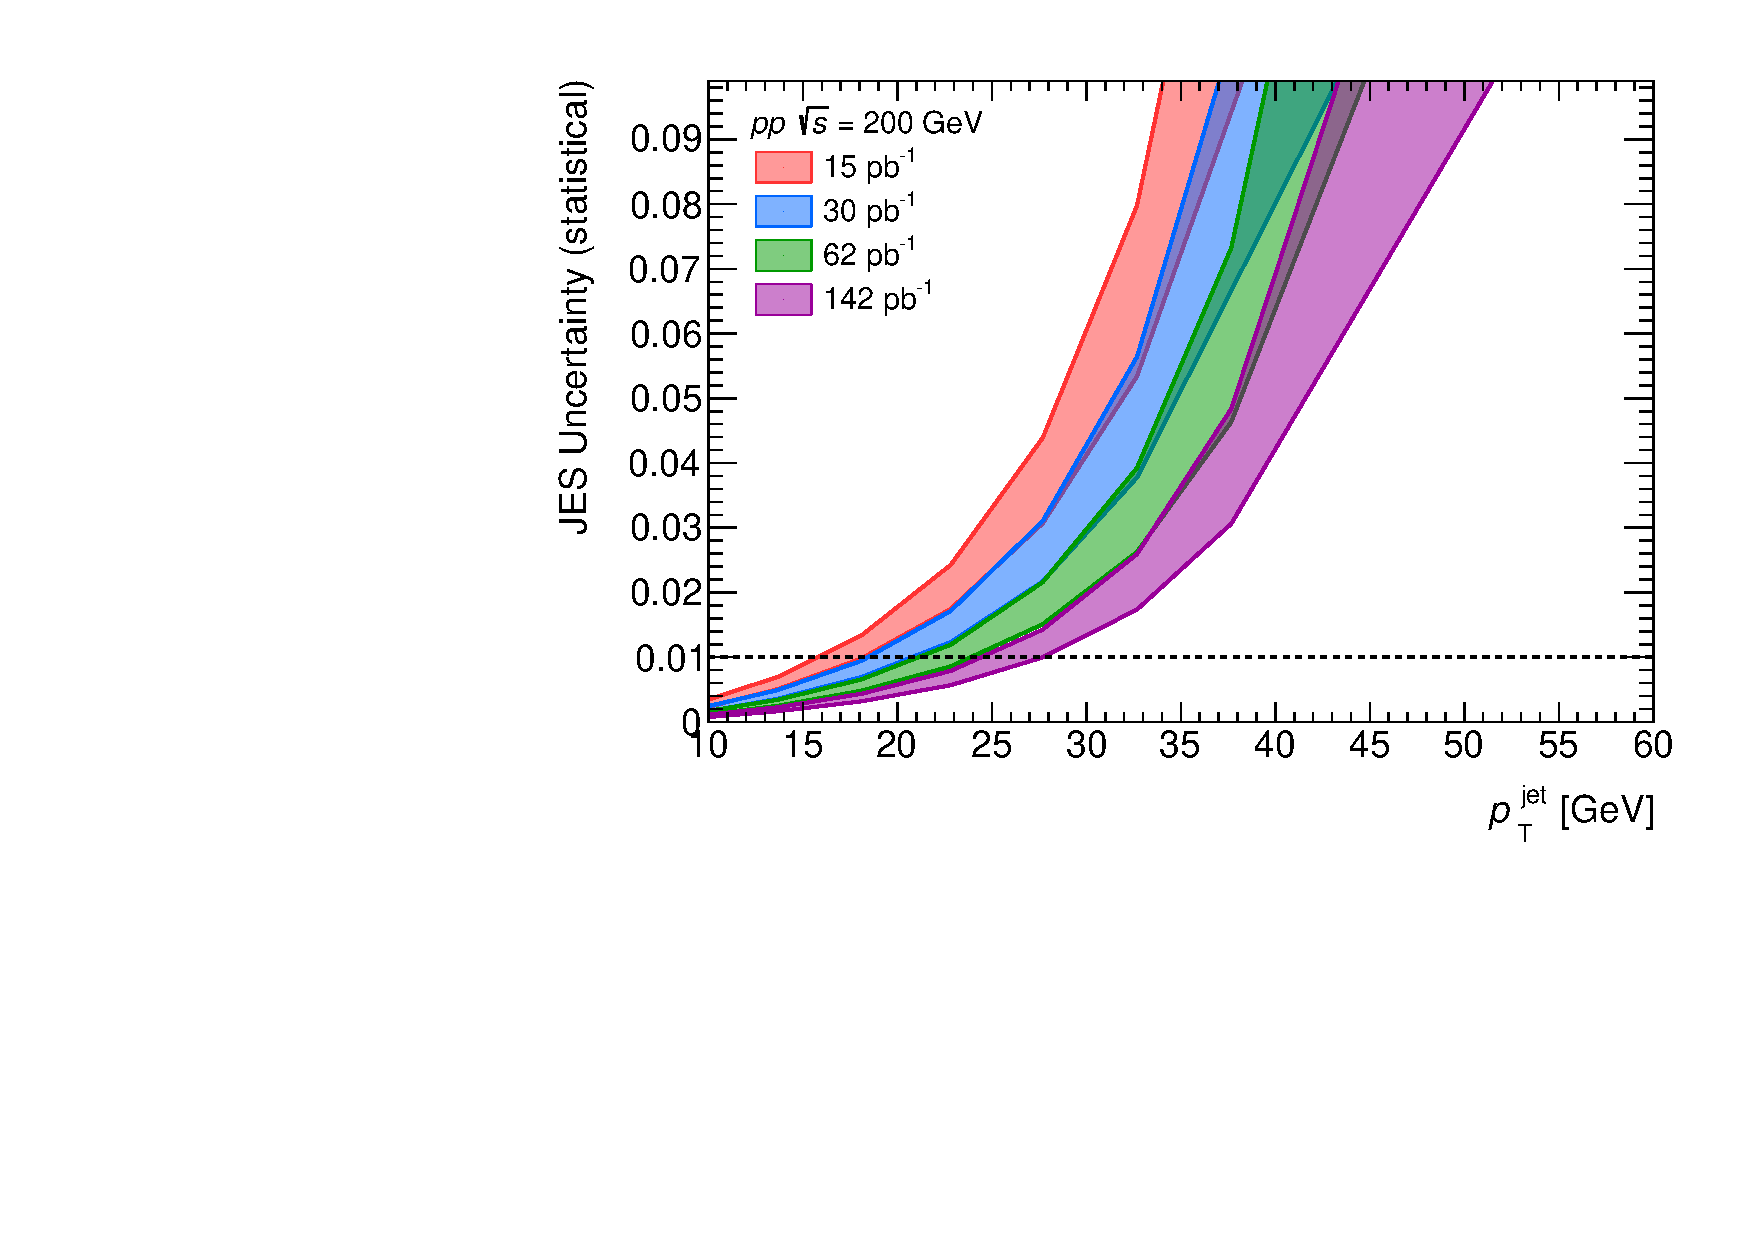
\includegraphics[width=0.8\linewidth]{figs/CompareSqrtsBUR.pdf}
    \caption{The projected sPHENIX statistical uncertainty contribution to the Jet Energy Scale (JES) uncertainty as determined from the ``golden channel'' via photon-jet direct balance studies.}
    \label{fig:jes}
\end{figure}

